\chapter{Systembeskrivelse}\label{Systembeskrivelse}
Formålet med Automatisk Ultralydsscanner er at gøre det muligt at lave en fuldautomatisk ultralydsscanninger af mamma til screening for brystkræft. En operatør med kendskab til ultralyd kan via en grafisk brugergrænseflade (GUI) betjene systemet, bestående af en PC Applikation installeret på en computer. Operatøren skal tænde for robotarmen og sikre, at 3D kamera er tilsluttet til computeren gennem 3D kameraets USB-kabel. Operatøren sikrer forbindelsen til robotarmen med et access point. Robotarmen er tilsluttet til access pointet gennem et ethernetkabel, og videre til computeren gennem et andet ethernetkabel fra access point til computeren.  

Robotarmen har på det yderste led påmonteret en ultralydsprobe, og robotarmen er placeret ved siden af briksen, hvor patienten skal ligge. 3D kameraet er monteret i loftet over briksen. Operatør guider patienten til at ligge på briksen og sikrer, at  brystområdet er indenfor intervallet og hovedet er udenfor intervallet. 

Operatør sørger for, at ultralydsscanneren er tændt, og gennem PC Applikation har operatøren mulighed for at 3D scanne en patients brystområde. PC Applikation processerer brystområdets form og position fra 3D kameraet og leverer informationen videre til robotarmen, som fører ultralysdsproben fra ultralydsscanneren rundt på brystområdet.  Operatøren kan følge med på ultralydsscannerens skærm under scanningen. 

Figur \ref{Systembeskrivelse} viser en oversigt over systemet og interaktionen mellem aktørerne. 

\begin{figure}[H]
    \centering
    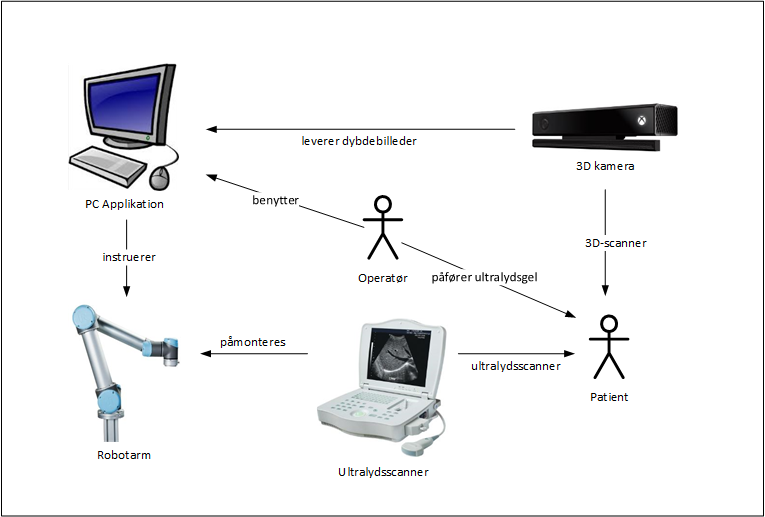
\includegraphics[width=0.67\textwidth]{figurer/d/Kravspecifikation/Systembeskrivelse}
    \caption{Systemoversigt}
    \label{Systembeskrivelse}
\end{figure}
\pagebreak
